% =============================================================================
% COPYRIGHT AND DISCLAIMER
% =============================================================================
% This file is provided as a convenience template for competition participants.
% By using it, you accept full responsibility for compliance with all applicable
% copyright, licensing, and usage rules of the Association for Computing
% Machinery (ACM) and of any LaTeX packages you load (including, without
% limitation, the "acmart" document class and related ACM materials).
%
% Consult ACM's official publication, template, and copyright policies before
% using this setup for any purpose other than this competition. Do not assume
% that this template may be reused, redistributed, or submitted elsewhere
% without independently verifying ACM's current rules.
%
% Use of the "acmart" class, the "sigconf" option, or ACM-style formatting in
% this template does NOT mean that this report, this competition, its organizers,
% or any resulting PDF is sponsored, endorsed, affiliated with, or published by
% ACM. ACM trademarks and branding remain the property of ACM.
%
% Template packages live in preamble.tex.
% Citations live in main.bib. Edit this file with your paper content.
% =============================================================================

\documentclass[sigconf]{acmart}
% =============================================================================
% Template setup — participants normally do not edit this file.
% Author content belongs in main.tex; citations belong in main.bib.
% \documentclass lives in main.tex so Overleaf does not treat this file as root.
% =============================================================================

% --- Competition / non-ACM-submission friendly rights metadata -------------
\setcopyright{none}
\settopmatter{printacmref=false}
\acmConference[Kaggle Competition]{Filament Segmentation Challenge}{2026}{\href{https://www.kaggle.com/competitions/filament-segmentation-2026}{kaggle.com/competitions/filament-segmentation-2026}}
\acmBooktitle{Competition Report}
\acmDOI{}
\acmISBN{}

% --- Author guidance text --------------------------------------------------
% \guide{...} is gray italic while \guideStyletrue; omitted from the PDF if false.
% Flip the switch in main.tex after % =============================================================================
% Template setup — participants normally do not edit this file.
% Author content belongs in main.tex; citations belong in main.bib.
% \documentclass lives in main.tex so Overleaf does not treat this file as root.
% =============================================================================

% --- Competition / non-ACM-submission friendly rights metadata -------------
\setcopyright{none}
\settopmatter{printacmref=false}
\acmConference[Kaggle Competition]{Filament Segmentation Challenge}{2026}{\href{https://www.kaggle.com/competitions/filament-segmentation-2026}{kaggle.com/competitions/filament-segmentation-2026}}
\acmBooktitle{Competition Report}
\acmDOI{}
\acmISBN{}

% --- Author guidance text --------------------------------------------------
% \guide{...} is gray italic while \guideStyletrue; omitted from the PDF if false.
% Flip the switch in main.tex after % =============================================================================
% Template setup — participants normally do not edit this file.
% Author content belongs in main.tex; citations belong in main.bib.
% \documentclass lives in main.tex so Overleaf does not treat this file as root.
% =============================================================================

% --- Competition / non-ACM-submission friendly rights metadata -------------
\setcopyright{none}
\settopmatter{printacmref=false}
\acmConference[Kaggle Competition]{Filament Segmentation Challenge}{2026}{\href{https://www.kaggle.com/competitions/filament-segmentation-2026}{kaggle.com/competitions/filament-segmentation-2026}}
\acmBooktitle{Competition Report}
\acmDOI{}
\acmISBN{}

% --- Author guidance text --------------------------------------------------
% \guide{...} is gray italic while \guideStyletrue; omitted from the PDF if false.
% Flip the switch in main.tex after \input{preamble}.
%
% Do not use \guide{...} for \email{...}.
\usepackage{xcolor}
\newif\ifguideStyle
\guideStyletrue
\newcommand{\guide}[1]{%
  \ifguideStyle
    {\color{gray!65}\itshape #1}%
  \fi
}

% --- Math ------------------------------------------------------------------
% Do NOT load amssymb (or amsfonts): acmart already loads newtxmath, which
% defines the same symbols (e.g. \Bbbk) and causes a conflict on Overleaf.
% amsmath is already provided by acmart; mathtools extends it.
\usepackage{mathtools}

% --- Figures ---------------------------------------------------------------
% graphicx is already loaded by acmart
\usepackage{subcaption}

% --- Tables ----------------------------------------------------------------
% booktabs is already loaded by acmart
\usepackage{tabularx}
\usepackage{multirow}

% --- Bibliography style is set in main.tex (ACM-Reference-Format) ----------
.
%
% Do not use \guide{...} for \email{...}.
\usepackage{xcolor}
\newif\ifguideStyle
\guideStyletrue
\newcommand{\guide}[1]{%
  \ifguideStyle
    {\color{gray!65}\itshape #1}%
  \fi
}

% --- Math ------------------------------------------------------------------
% Do NOT load amssymb (or amsfonts): acmart already loads newtxmath, which
% defines the same symbols (e.g. \Bbbk) and causes a conflict on Overleaf.
% amsmath is already provided by acmart; mathtools extends it.
\usepackage{mathtools}

% --- Figures ---------------------------------------------------------------
% graphicx is already loaded by acmart
\usepackage{subcaption}

% --- Tables ----------------------------------------------------------------
% booktabs is already loaded by acmart
\usepackage{tabularx}
\usepackage{multirow}

% --- Bibliography style is set in main.tex (ACM-Reference-Format) ----------
.
%
% Do not use \guide{...} for \email{...}.
\usepackage{xcolor}
\newif\ifguideStyle
\guideStyletrue
\newcommand{\guide}[1]{%
  \ifguideStyle
    {\color{gray!65}\itshape #1}%
  \fi
}

% --- Math ------------------------------------------------------------------
% Do NOT load amssymb (or amsfonts): acmart already loads newtxmath, which
% defines the same symbols (e.g. \Bbbk) and causes a conflict on Overleaf.
% amsmath is already provided by acmart; mathtools extends it.
\usepackage{mathtools}

% --- Figures ---------------------------------------------------------------
% graphicx is already loaded by acmart
\usepackage{subcaption}

% --- Tables ----------------------------------------------------------------
% booktabs is already loaded by acmart
\usepackage{tabularx}
\usepackage{multirow}

% --- Bibliography style is set in main.tex (ACM-Reference-Format) ----------


% Guide styling: \guideStyletrue = show gray italic hints; \guideStylefalse = omit them
% \guideStyletrue
\guideStylefalse

\begin{document}

\title{FilaNet: A Deformable Edge-Attention U-Net with Hysteresis Instance Extraction}
\subtitle{A Solution to the Solar Filament Segmentation Challenge 2026}


\author{Paschalis Dompoudis}
\affiliation{
  \country{Greece}
}
\email{paschalis.dompoudis@proton.me}

\begin{abstract}
    This report describes our solution to the Solar Filament Segmentation Challenge~2026, a Kaggle competition on automatic segmentation of solar filaments in GONG H-$\alpha$ observations. FilaNet is a U-Net in the style of EdgeAttNet: its bottleneck self-attention is guided by a learned edge map instead of positional encodings, and every $3\times3$ convolution is deformable, so the kernels can follow thin, curved filaments. It processes full $2048\times2048$ frames after a preprocessing step that finds the solar limb and flattens limb darkening and clouds. It is trained in two stages: on $512$-pixel windows, then on full frames with an auxiliary centreline output and extra loss weight on small filaments. Because the competition scores individual filaments, hysteresis thresholding, eight-fold test-time augmentation and merging of nearby fragments turn the probability map into instances. On 106 held-out photographs the pipeline reaches a Panoptic Quality of 0.391 at its selected operating point. Split-half cross-validation, which removes the optimism of choosing that point on the same photographs, gives 0.386. For comparison, one human annotator scored against another reaches 0.33.
\end{abstract}

\maketitle

\ifguideStyle
\noindent{\color{gray!65}\itshape
Guide mode is on.}
\par\medskip
\fi

% ==================================== %
%              INTRODUCTION            %
% ==================================== %
\section{Introduction}
    This report goes over the details of our submitted solution to the Solar Filament Segmentation Challenge~2026 \cite{filament-segmentation-2026}. The challenge, launched on July~10,~2026, is organized by the Earth-Space AI Research (ESAIR) Lab\footnote{\href{https://www.esairlab.com/home}{www.esairlab.com/}}. This challenge utilizes the MAGFiLO dataset for evaluation of the segmentation algorithms \cite{ahmadzadeh2024dataset}.

    The leaderboard scores Panoptic Quality (PQ) \cite{kirillov2019panoptic} over individual filaments. A predicted filament counts as a true positive (TP) only if its IoU with an annotated one exceeds 0.5, and $\mathrm{PQ}=\sum_{\mathrm{TP}}\mathrm{IoU}/(|\mathrm{TP}|+\tfrac12|\mathrm{FP}|+\tfrac12|\mathrm{FN}|)$. Each test photograph receives one prediction, which is scored against every annotator who labelled it. This shaped three decisions. We segment at full resolution, because filaments are a median 13~px wide. We post-process the probability map specifically for instance-level matching. And we judge every change by the PQ it earns on held-out photographs, with an uncertainty estimate attached, rather than by the public leaderboard (Section~\ref{sec:evaluation}). Code, weights and a notebook that reproduces the submission are in the accompanying repository.

% ==================================== %
%              METHODOLOGY             %
% ==================================== %
\section{Methodology}\label{sec:methodology}

\begin{figure*}[t]
  \centering
  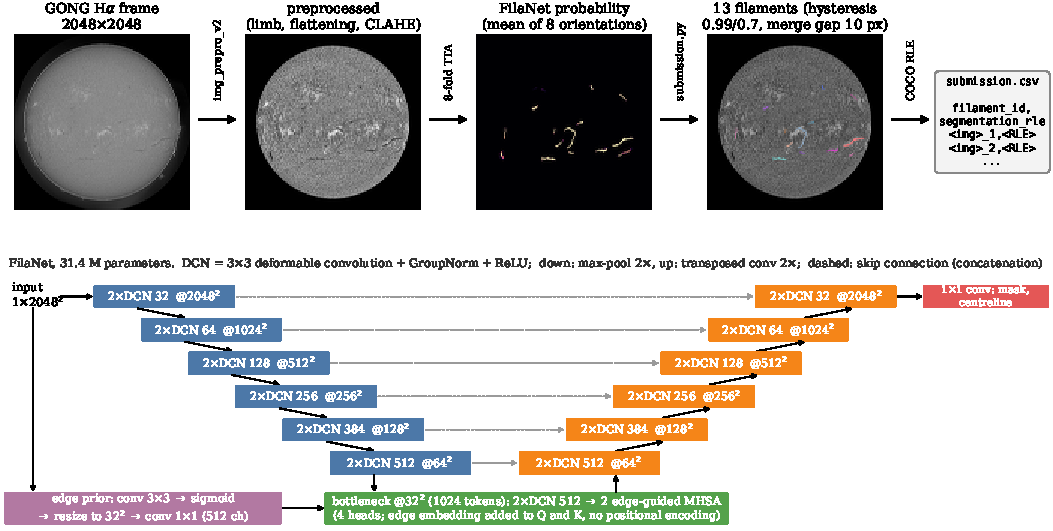
\includegraphics[width=\textwidth]{figures/pipeline.pdf}
  \caption{End-to-end pipeline on a held-out validation photograph (top) and the FilaNet architecture (bottom).}
  \label{fig:pipeline}
\end{figure*}

\subsection{Data and splits}
The training set has 707 photographs and 1154 annotator-images: 411 photographs were annotated by one person, 145 by two and 151 by three, with 37 annotators and 8199 filament polygons in total. We split by \emph{photograph}, so that two annotations of the same image never fall on different sides: 601 photographs train the model and 106 (175 annotator-images, 1387 filaments) are held out for model selection and every number in Section~\ref{sec:evaluation}. The released model never saw the held-out photographs. Where a training photograph has several annotators, the target is the union of their masks, so that each photograph appears once per epoch with one target. Training on each annotator's copy separately shows the network contradictory masks of the same image. The test set has 180 photographs.

\subsection{Preprocessing}
GONG frames differ in brightness, limb darkening, haze and cloud. Each frame goes through five steps (Fig.~\ref{fig:pipeline}):
(i)~\emph{Limb detection.} An Otsu threshold gives a rough centre. The frame is unwrapped to polar coordinates, and on each of 720 rays the limb is the steepest intensity drop within $\pm5\%$ of the known solar radius (907~px). A circle is then fitted with iterative rejection of outliers. Restricting the search radius matters: without it, the outer edge of an atmospheric halo, which is often the stronger edge, was taken for the limb in 14\% of training frames.
(ii)~Division by the median radial intensity profile, which removes limb darkening.
(iii)~Division by a coarse two-dimensional median background (kernel $\approx$250~px), which removes clouds and gradients, in the spirit of median-filter flattening \cite{menshchikov2017getimages}.
(iv)~A \emph{fixed} intensity window: ratios 0.6--1.4 map to 0--255 in every frame, followed by a light Gaussian blur.
(v)~CLAHE \cite{zuiderveld1994clahe} inside the disk (clip 1.5, $8\times8$ tiles). Pixels beyond $0.98R$ are set to zero.
All 887 training and test frames pass the limb check.

\begin{figure*}[t]
  \centering
  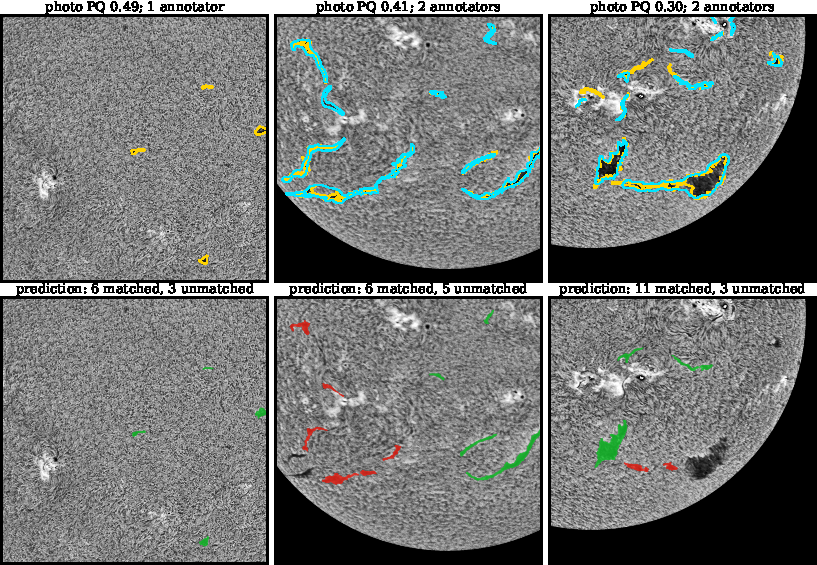
\includegraphics[width=0.86\textwidth]{figures/examples.pdf}
  \caption{Held-out photographs at the 80th, 50th and 20th percentile of per-photograph PQ (among those with $\geq$8 annotated filaments), cropped to the annotated region. Top: annotators' outlines, one colour per annotator. Bottom: submitted filaments, green if they match some annotator's filament at IoU~$>0.5$, red otherwise. Counts in the titles are for the whole frame.}
  \label{fig:examples}
\end{figure*}

\subsection{Network}
FilaNet follows EdgeAttNet \cite{solomon2025edgeattnet}, a U-Net \cite{ronneberger2015unet} whose bottleneck runs multi-head self-attention, with a learned edge map added to the queries and keys in place of positional encodings. The edge map is a $3\times3$ convolution and a sigmoid on the input, resized to the token grid and projected by a $1\times1$ convolution. Our main change replaces \emph{every} $3\times3$ convolution in the encoder, bottleneck and decoder with a deformable convolution \cite{dai2017deformable}. Its sampling offsets are predicted per pixel, so a kernel can bend along a thin, curved filament or barb, as deformable U-Nets do for retinal vessels \cite{jin2018dunet}.

To process whole $2048\times2048$ frames, the encoder has six stages of two deformable convolutions each, with widths 32--64--128--256--384--512 and max-pooling between stages. The bottleneck therefore attends over a $32\times32$ grid of 1024 tokens (two attention blocks, four heads, dropout 0.1). The decoder mirrors the encoder with transposed convolutions and skip connections. We use GroupNorm \cite{wu2018group} instead of BatchNorm. With BatchNorm, statistics accumulated on training windows (mean intensity 0.47, 9\% off-disk) and applied to full frames (0.30, 41\%) inflated predicted foreground from 0.6\% to 52\%. A $1\times1$ head outputs two channels: the filament mask, and the filament centreline as an auxiliary target that is never submitted. The head bias starts at the log-odds of the 0.36\% foreground rate. The network has 31.4\,M parameters.

\subsection{Loss}
The mask channel is trained with
$\mathcal{L}_{\mathrm{mask}} = 0.7\,(1-T_{\beta}) + 0.3\,(1-\mathrm{clDice}) + \mathrm{BCE}_w$,
where $T_{\beta}$ is the soft Tversky index \cite{salehi2017tversky} with $\beta=0.7$, which penalises missed pixels more than false alarms because our errors were dominated by misses. clDice \cite{shit2021cldice} rewards connected centrelines, using a soft skeleton of 47 iterations to reach the widest filament. The BCE term is essential. Both region terms have practically no gradient on the 99.6\% background pixels, and without BCE the first run converged to predicting 99.99\% foreground. In stage~2, $\mathrm{BCE}_w$ gives each pixel the weight $w=\mathrm{clip}(\sqrt{1500/A},1,4)$, where $A$ is the area of the filament it belongs to. This counteracts a pixel loss's bias towards large filaments, since PQ counts every filament once. The centreline channel targets the annotated spines, drawn 3~px wide and clipped to the mask, with BCE plus soft Dice at weight 0.5.

\subsection{Training}
\emph{Stage~1} (30 epochs): random $512\times512$ windows, 70\% of them centred on a filament pixel, batch~8, random rotation by multiples of $90^\circ$ and mirroring. AdamW \cite{loshchilov2019adamw} with learning rate $10^{-4}$ and weight decay 0.01, one warm-up epoch, then cosine decay \cite{loshchilov2017sgdr} to $10^{-6}$.
\emph{Stage~2} (3 epochs from stage~1): \emph{full} frames, so that the attention sees the 1024-token context used at test time. Batch~1 with 4 accumulated steps, learning rate $3\times10^{-5}$ with cosine decay, and the centreline and size-weighting terms added.
Validation PQ selects the checkpoint in both stages. Training ran on one 16\,GB RTX A4000. A full frame needs 21\,GB with gradients, so Windows pages to host memory and an epoch takes $\approx$3.3\,h. Mixed precision made this worse. Validation PQ was still rising at the end of stage~2 (Fig.~\ref{fig:eval}a).

\begin{figure*}[t]
  \centering
  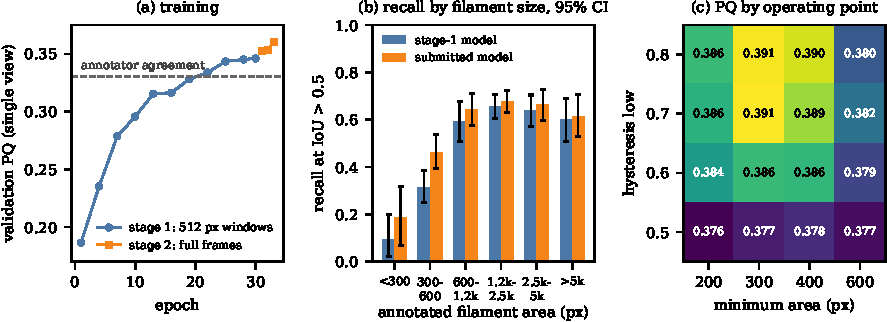
\includegraphics[width=\textwidth]{figures/evaluation.pdf}
  \caption{(a) Validation PQ during training (single view, a fixed coarse grid of eight operating points; the dashed line is annotator--annotator agreement). (b) Fraction of annotated filaments matched at IoU~$>0.5$, by size, with 95\% bootstrap intervals over photographs. (c) PQ of the final model over the post-processing grid (merge gap 10~px, best high threshold per cell).}
  \label{fig:eval}
\end{figure*}

\subsection{Inference and post-processing}
Each test frame is predicted in all eight orientations of the square, and the probability maps are rotated back and averaged (12\,s per frame). Instances are then extracted in three steps.
(i)~\emph{Hysteresis} \cite{canny1986edge}: a filament is an 8-connected region of pixels with $p\geq0.7$ that contains at least one pixel with $p\geq0.99$. The confident core decides \emph{whether} a filament exists, and the lower threshold how far it extends. A single threshold must trade one against the other.
(ii)~Regions under 300~px are dropped.
(iii)~\emph{Fragment merging}: the network sometimes breaks a filament into a chain of pieces that individually miss IoU~0.5, so pieces within 10~px of each other become one instance, keeping only their own pixels.
The values $(0.99, 0.7, 300, 10)$ come from a grid of 144 settings on the validation photographs. Fig.~\ref{fig:eval}c shows that neighbouring settings score within 0.005 of it. Each instance is written as a COCO run-length encoding.

% ==================================== %
%              EVALUATION              %
% ==================================== %
\section{Evaluation}\label{sec:evaluation}

\paragraph{Protocol.}
We score the 106 held-out photographs with a line-by-line port of the organisers' PQ code. Each photograph is predicted once and scored against each of its annotators, and the counts are pooled. Uncertainty comes from two resampling schemes. A \emph{bootstrap} over photographs (4000 resamples \cite{efron1993bootstrap}) gives confidence intervals at a fixed setting. Repeated \emph{split-half cross-validation} (1000 random halvings) chooses the post-processing setting on one half and scores it on the other, which yields a \emph{held-out} PQ free of the optimism of tuning on the scored photographs. Partitions are shared across rows, so differences are paired. We did not rely on the public leaderboard to compare models: two of our earlier models that are indistinguishable on validation (difference $-0.0001$, 95\% CI $\pm0.015$) scored 0.32 and 0.28 there. As a reference, a held-out human annotator scored against another annotator of the same photographs reaches PQ~0.33.

\begin{table}[t]
  \caption{Ablation on the 106 held-out photographs. Held-out PQ is the mean over 1000 split-half partitions (setting chosen on one half, scored on the other) $\pm$ its standard deviation. $\Delta$ is the paired change from the previous row (stage-1 model: relative to the submitted row), with its 5--95\% range over partitions.}
  \label{tab:ablation}
  \footnotesize\setlength{\tabcolsep}{3pt}
  \begin{tabular}{@{}lccc@{}}
    \toprule
    Pipeline & In-sample & Held-out & $\Delta$ [5\%, 95\%] \\
    \midrule
    One view, single threshold & 0.364 & 0.359\,$\pm$\,0.013 & -- \\
    \;+ hysteresis             & 0.368 & 0.363\,$\pm$\,0.013 & $+$0.005 [$-$0.003, $+$0.012] \\
    \;+ fragment merging       & 0.378 & 0.372\,$\pm$\,0.013 & $+$0.008 [$-$0.002, $+$0.018] \\
    \;+ 8-fold TTA (submitted) & \textbf{0.391} & \textbf{0.386}\,$\pm$\,0.013 & $+$0.014 [$+$0.003, $+$0.025] \\
    \midrule
    Stage-1 model, full pipeline & 0.375 & 0.372\,$\pm$\,0.013 & $-$0.014 [$-$0.024, $-$0.003] \\
    \bottomrule
  \end{tabular}
\end{table}

\begin{table}[t]
  \caption{The submitted pipeline at its selected setting, with 95\% bootstrap intervals over photographs, against the stage-1 model at its own best setting.}
  \label{tab:final}
  \footnotesize\setlength{\tabcolsep}{3pt}
  \begin{tabular}{@{}lccc@{}}
    \toprule
     & PQ & SQ & RQ \\
    \midrule
    Submitted & \textbf{0.391} [0.365, 0.414] & 0.658 [0.649, 0.666] & 0.595 [0.559, 0.627] \\
    Stage 1   & 0.375 [0.347, 0.399] & 0.657 [0.649, 0.664] & 0.571 [0.531, 0.606] \\
    \bottomrule
  \end{tabular}\\[2pt]
  \footnotesize Submitted: TP 839, FP 596, FN 548. Paired PQ gain over stage~1: $+$0.016, 95\% CI [$+$0.007, $+$0.025].
\end{table}

\paragraph{Results.}
Table~\ref{tab:ablation} builds the pipeline up one step at a time. Each step helps, and the gains add up to $+0.027$ held-out PQ over a single-threshold baseline. Hysteresis and fragment merging are individually small (the 5--95\% ranges include zero) but consistent in sign, and test-time augmentation is the largest single step. The stage-2 fine-tuning adds $+0.014$ over the stage-1 model under the same pipeline (Table~\ref{tab:ablation}). The bootstrap at the selected setting puts that gain at $+0.016$, with a 95\% interval of $[+0.007, +0.025]$ that excludes zero (Table~\ref{tab:final}). The gain comes from detection, not from outline quality: SQ is unchanged at 0.66, while recognition quality (RQ) rises from 0.571 to 0.595, with 73 more true positives and 73 fewer misses. Fig.~\ref{fig:eval}b shows where those detections come from. Recall on filaments of 300--600~px rises from 0.31 to 0.46, which is what the size-weighted loss targeted. Fig.~\ref{fig:examples} shows typical outcomes.

\paragraph{Strengths.}
The pipeline's held-out PQ (0.386) exceeds the PQ of one human annotator scored against another on the same photographs (0.33). That reference is measured only on photographs with several annotators, so the comparison is indicative, but the label noise clearly bounds what this metric can reward. Its operating point lies on a broad plateau (Fig.~\ref{fig:eval}c), so the selected setting is not a lucky outlier. The pipeline is also fully reproducible: a fixed preprocessing, one network and deterministic post-processing.

\paragraph{Weaknesses.}
(i)~\emph{Small filaments.} Only 19\% of annotated filaments under 300~px are matched, and 46\% of those of 300--600~px (Fig.~\ref{fig:eval}b). Some fall below the 300~px area filter, and most are faint features that annotators themselves disagree on.
(ii)~\emph{Large filaments are found but cut short.} 95.5\% of filaments over 2500~px are touched by a prediction, but only 65\% are matched, because the matched instance covers a median of 77\% of the outline and an under-segmented or fragmented instance falls below IoU~0.5 (red instances in Fig.~\ref{fig:examples}, middle and right).
(iii)~\emph{False positives} (596) are about as numerous as misses (548). Some are fragments of annotated filaments that stay below IoU~0.5, as in (ii). Others are faint structures that no annotator of that photograph outlined, a judgement on which annotators themselves differ.
(iv)~\emph{Cost.} Deformable convolutions at full resolution make training slow on a 16\,GB GPU, which limited us to 33 epochs in total, and test-time augmentation makes inference eight times slower (12\,s per frame).

\paragraph{Possible improvements.}
(i)~Retrain on all 707 photographs, since the 106 held out here cost 15\% of the data. (ii)~Continue stage~2: full-frame training still improved at every epoch but costs 3.3\,h per epoch on our hardware, which more GPU memory would remove. (iii)~Replace connected-component instances with a learned instance head, which would separate touching filaments and join broken ones by learning rather than by a fixed gap. (iv)~Model the annotator disagreement explicitly, for instance with soft multi-annotator targets, because label noise and not the network sets the ceiling of this metric.


% ==================================== %
%            ACKNOWLEDGMENT            %
% ==================================== %
\section{Acknowledgment}\label{sec:acknowledgment}
    % Do not change
    The organization of the Filament Segmentation Challenge 2026 is partially supported by the U.S. National Science Foundation (NSF) under Grant No. 2209912 and 2433781, directorate for Computer and Information Science and Engineering (CSE), and Office of Advanced Cyberinfrastructure (OAC), and Grant No. 2511630, AST Division Of Astronomical Sciences and MPS Directorate for Mathematical and Physical Sciences.

    The Filament Segmentation Challenge 2026 is sponsored by the U.S. National Science Foundation (NSF) National Solar Observatory (NSO).

    This work utilizes GONG data obtained by the NSO Integrated Synoptic Program, managed by the National Solar Observatory, which is operated by the Association of Universities for Research in Astronomy (AURA), Inc. under a cooperative agreement with the National Science Foundation and with contribution from the National Oceanic and Atmospheric Administration. The GONG network of instruments is hosted by the Big Bear Solar Observatory, High Altitude Observatory, Learmonth Solar Observatory, Udaipur Solar Observatory, Instituto de Astrofísica de Canarias, and Cerro Tololo Interamerican Observatory.

\bibliographystyle{ACM-Reference-Format}
\bibliography{main,references}

\end{document}
